\chapter{Revisão Teórica}\label{cap_revisao}

\section{Arquitetura de Computadores}
{
    Para nos comunicarmos, necessitamos de uma linguagem, e no caso dos
    brasileiros, essa linguagem é o português. Como toda linguagem, o português
    possui sua gramática e dicionário que lhe dá estrutura e sentido. Línguas
    humanas como o português, inglês e espanhol são chamadas de linguagens
    naturais, e evoluíram naturalmente a partir do uso e
    repetição.~\cite{lyons1991natural}

    Por causa da excelente capacidade de interpretação e adaptação da mente
    humana, somos capazes de criar e entender novos dialetos que não seguem as
    regras formais das linguagens naturais que conhecemos. Porém, fora da
    comunicação casual é importante e às vezes obrigatório que nos expressemos
    sem ambiguidade. Línguas artificiais como a notação matemática e linguagens
    de programação possuem semântica e sintaxe mais rígidas para garantir que
    a mensagem transmitida seja interpretada da maneira correta. Sem essa
    rigidez, os computadores de hoje não seriam capazes de entender nossos
    comandos.
}

{
    Para a comunicação com o processador de um computador, utilizamos mensagens
    chamadas de instruções, e o conjunto dessas instruções é chamado de
    Arquitetura do Conjunto de Instruções (\textit{ISA}). Um processador só é
    capaz de entender as mensagens que obedecem as regras semânticas e
    sintáticas de sua \textit{ISA}, e qualquer instrução que fuja das suas
    regras causará um erro de execução ou realizará uma tarefa diferente da
    pretendida. A linguagem de máquina é considerada de baixo nível pois
    apresenta pouca ou nenhuma abstração em relação à arquitetura.

    As instruções são passadas para o processador na forma de código de máquina,
    sequências de dígitos binários que correspondem aos níveis lógicos do
    circuito. Para melhorar o entendimento do código e facilitar o
    desenvolvimento, uma outra representação é utilizada, o \textit{assembly}.
    Um código \textit{assembly} é transformado em código de máquina por um
    programa montador, (\textit{assembler}), e o processo inverso é realizado
    por um \textit{disassembler}. As linguagens \textit{assembly}, dependendo do
    \textit{assembler} utilizado, permitem o uso de macros de substituição e
    pseudo instruções (determinadas instruções que não existem na \textit{ISA}
    que são expandidas em instruções válidas pelo montador) e são totalmente
    dependentes da arquitetura do processador, o que normalmente impede que o
    mesmo código seja executado em arquiteturas diferentes.
}

{
    A Figura~\ref{fig:cpu_abstraction} é uma representação simplificada de um
    processador. A unidade de controle lê uma instrução da memória e a
    decodifica; o circuito de lógica combinacional lê os dados dos
    registradores, entrada e memória conforme necessário, executa a instrução
    decodificada e escreve no banco de registradores, na memória de dados ou
    na saída se for preciso; a unidade de controle lê uma nova instrução e o
    ciclo se repete até o fim do programa. A posição de memória da instrução
    que está sendo executada fica armazenada em um registrador especial chamado
    de Contador de Programa (\textit{PC}). Algumas instruções modificam o
    \textit{PC} condicionalmente ou diretamente, criando a estrutura para
    saltos, laços e chamada/retorno de funções.
}

\begin{figure}[H]
\centering
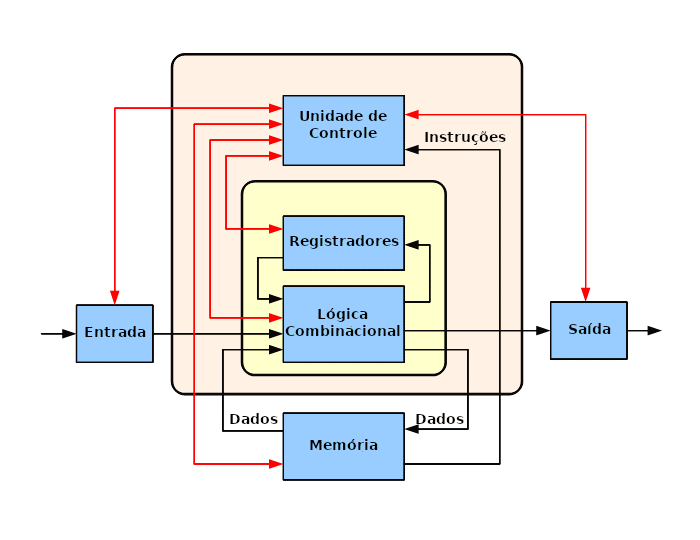
\includegraphics[width=.7\linewidth]
    {../images/ABasicComputer.png}
    \caption[Abstração da arquitetura de um computador]
    {Abstração da arquitetura de um
        computador.~\cite{wikimedia2015basiccpu}}\label{fig:cpu_abstraction}
\end{figure}

{
    Historicamente, as arquiteturas são divididas em \textit{ISAs}
    \textit{RISC} e \textit{CISC}. Na atualidade, a diferença entre elas é que
    as \textit{ISAs RISC} acessam a memória por instruções de
    \textit{load/store}, enquanto as \textit{CISC} podem acessar a memória
    diretamente em uma instrução de operação lógica ou aritmética.

    Algumas arquiteturas \textit{RISC} notáveis são a \textit{RISC-V}, objeto de
    estudo desse trabalho, a \textit{ARM} e a \textit{MIPS}. Quanto às
    \textit{CISC}, a \textit{x86} e sua extensão de 64 \textit{bits}, a
    \textit{AMD64}, são as mais conhecidas.
}

    \subsection{Arquitetura MIPS}
    {}

    \subsection{Arquitetura ARM}
    {}

    \subsection{Arquitetura x86}
    {}

    \subsection{Arquitetura AMD64}
    {}

    \subsection{Arquitetura RISC-V}
    {
        A \textit{ISA RISC-V} é uma arquitetura modular, sendo o módulo base de
        operações com inteiros mandatório em qualquer implementação. Os demais
        módulos são extensões de uso opcional. A arquitetura não suporta
        \textit{branch delay slots} e aceita instruções de tamanho variável. A
        codificação das instruções de tamanho variável é mostrada na
        Figura~\ref{fig:riscv_var_length}. As instruções presentes no módulo
        base correspondem ao mínimo necessário para emular por
        \textit{software} as demais extensões (com exceção das operações
        atômicas).
    }

    \begin{figure}[H]
    \centering
        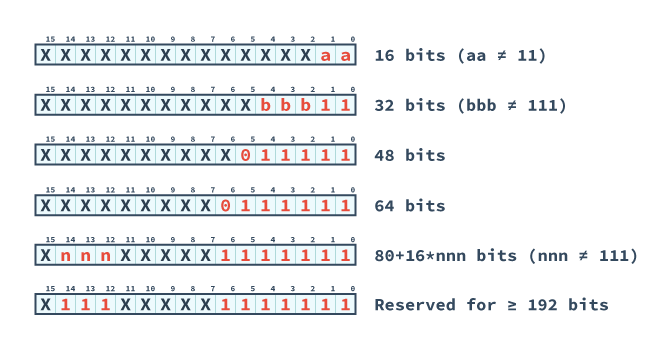
\includegraphics[width=1\linewidth]{../images/RV_InstructionLength.png}
        \caption{Codificação de instruções de tamanho variável da arquitetura
                    \textit{RISC-V}}\label{fig:riscv_var_length}
    \end{figure}

    {
        A nomenclatura do conjunto de instruções implementado segue a
        seguinte estrutura:
    }

    \begin{itemize}[leftmargin=20mm]
        \item {As letras ``RV'';}
        \item {A largura dos registradores do módulo Inteiro;}
        \item {A letra ``I'' representando a base Inteira. Caso o subconjunto
                Embarcado (\textit{Embedded}) seja implementado, substitui-se
                pela letra ``E'';}
        \item {Demais letras identificadoras de módulos opcionais.}
    \end{itemize}

    {
        Assim, uma implementação com registradores de 32 bits somente com o
        módulo base de Inteiros é denominado ``RV32I''.
    }

        \subsubsection{Módulo Inteiro}
        {
            O módulo Inteiro é o módulo base da arquiterura. O \textit{design} de sua
            especificação visa reduzir o \textit{hardware} necesário para uma
            implementação mínima, bem como ser um alvo de compilação satisfatório.
        }

        {
            Diferente de outras arquiteturas como a \textit{ARM}, as instruções de
            multiplicação e divisão não fazem parte do conjunto básico uam vez que
            necessitam de circuito especializado e por isso encarecem o desenvolvimento
            e produção dos processadores.
        }

        {
            Para sistemas embarcados com restrições mais severas de tamanho, custo,
            potência, etc o módulo base I pode ser substituído por um \textit{subset},
            o módulo E. Porém, nenhuma das demais extensões pode ser usada em conjunto
            com o módulo E.
        }

        \subsubsection{Extensões}
            \paragraph{Extensão M}
            {
                A extensão M implementa as operações de multiplicação e divisão de
                números inteiros.
            }

            \paragraph{Extensão A}
            {
                A extensão A implementa instruções de acesso atômico a memória.
                Instruções atômicas mantém a coerência da memória em sistemas
                preemptivos e paralelos.
            }

            \paragraph{Extensão F}
            {
                A extensão F implementa as isntruções de ponto flutuante IEEE 754 de
                precisão simples, bem como o banco de registradores especializado para
                operações com ponto flutuante.
            }

            \paragraph{Extensão D}
            {
                A extensão D implementa as instruções de ponto flutuante IEEE 754 de
                precisão dupla. Ela é um incremento à extensão F, sendo esta de
                implementação obrigatória para se poder implementar a extensão D.
            }

            \paragraph{Outras Extensões}
            {
                Outras extensões são previstas na especificação da arquitetura, e.g.
                a extensão C para instruções comprimidas (16 bits).
            }

            {
                A arquitetura prevê a expansão de extensões, com alguns
                \textit{opcodes} sendo reservados para essa finalidade. Desse modo,
                instruções proprietárias e/ou customisadas podem ser adicionadas.
            }

        \subsubsection{Arquitetura Privilegiada}
        {
            Para a \textit{ISA RISC-V}, existem quatro níveis de privilégio de acesso,
            sendo eles o de usuário (módulo I e extensões), de máquina
            (\textit{syscalls}) de supervisor (sistema operacional) e hipervisor
            (virtualização).
        }

        \subsubsection{Formatos de Instruções}
        {
            As instruções da arquitetura podem ser separadas em subgrupos de acordo com
            os operadores necessários para o processador interpretá-la. A
            Figura~\ref{fig:riscv_formats} apresenta os formatos das instruções do
            módulo I da \textit{ISA RISC-V}, e, para efeitos de comparação, a
            Figura~\ref{fig:mips_formats} mostra os formatos de instruções equivalentes
            na arquitetura MIPS32.
        }

        \begin{figure}[H]
        \centering
            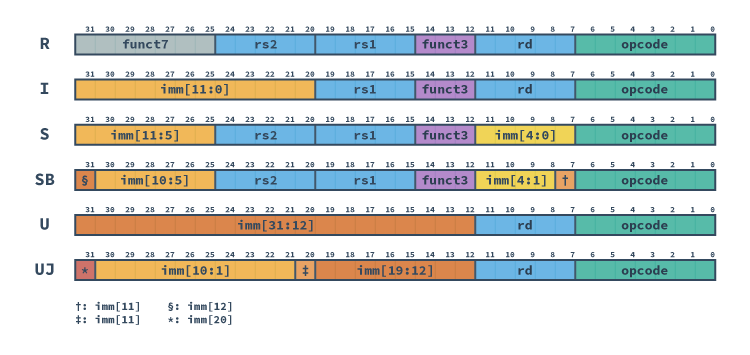
\includegraphics[width=1\linewidth]{../images/RV_Formats.png}
            \caption{Formatos de Instruções da \textit{ISA RISC-V}
                }\label{fig:riscv_formats}
        \end{figure}

        \begin{figure}[H]
        \centering
            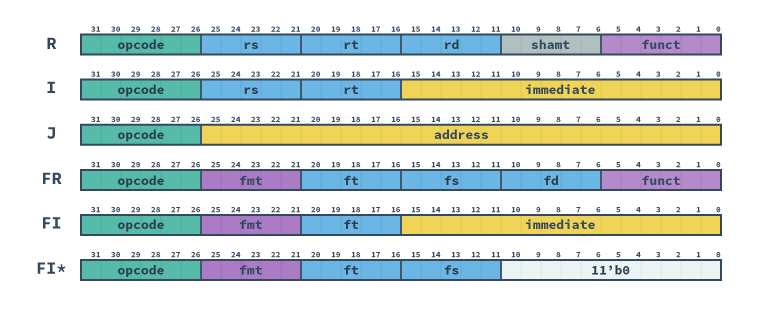
\includegraphics[width=1\linewidth]{../images/MIPS_Formats.png}
            \caption{Formatos de Instruções da \textit{ISA MIPS32}
                }\label{fig:mips_formats}
        \end{figure}

        \subsubsection{Formatos de Imediatos}
        {
            Os imediatos são operandos descritos na própria instrução em vez de estar
            contido em um registrador. Como os operandos necessitam ter a mesma largura
            que o banco de registradores, algumas regras são utilizadas para gerar os
            operandos imediatos. As figuras a seguir mostram a formação de cada tipo de
            imediato dos formatos da Figura~\ref{fig:riscv_formats}.
        }

        \begin{figure}[H]
        \centering
            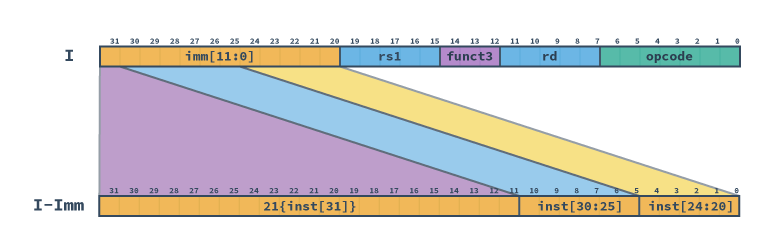
\includegraphics[width=1\linewidth]{../images/RV_I_Imm.png}
            \caption{Formação do Imediato de tipo I
                }\label{fig:riscv_i_imm}
        \end{figure}

        \begin{figure}[H]
        \centering
            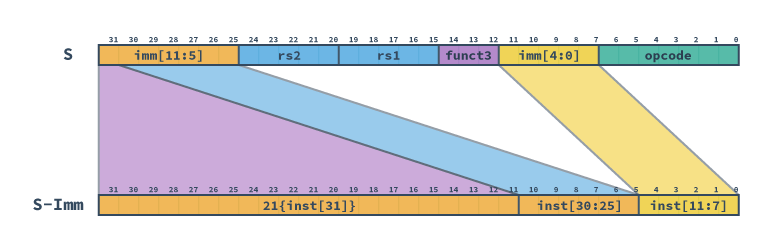
\includegraphics[width=1\linewidth]{../images/RV_S_Imm.png}
            \caption{Formação do Imediato de tipo S
                }\label{fig:riscv_s_imm}
        \end{figure}

        \begin{figure}[H]
        \centering
            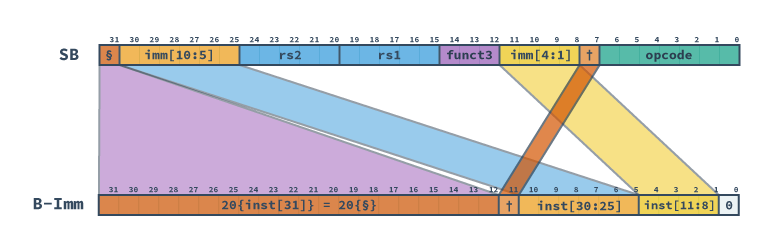
\includegraphics[width=1\linewidth]{../images/RV_B_Imm.png}
            \caption{Formação do Imediato de tipo B
                }\label{fig:riscv_b_imm}
        \end{figure}

        \begin{figure}[H]
        \centering
            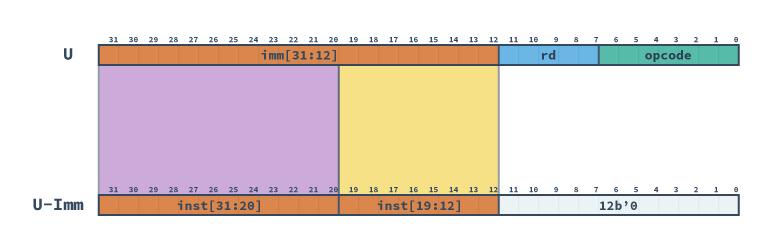
\includegraphics[width=1\linewidth]{../images/RV_U_Imm.png}
            \caption{Formação do Imediato de tipo U
                }\label{fig:riscv_u_imm}
        \end{figure}

        \begin{figure}[H]
        \centering
            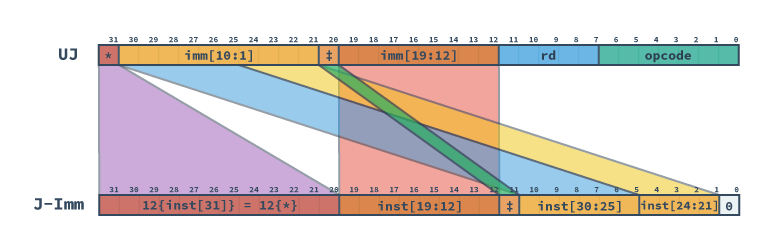
\includegraphics[width=1\linewidth]{../images/RV_J_Imm.png}
            \caption{Formação do Imediato de tipo J
                }\label{fig:riscv_j_imm}
        \end{figure}

        {
            Para efeitos comparativos, a Figura~\ref{fig:mips_immediates} mostra a
            formação de imediatos na arquitetura MIPS32.
        }

        \begin{figure}[H]
        \centering
            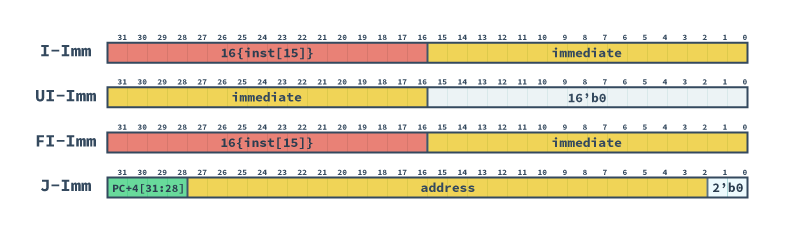
\includegraphics[width=1\linewidth]{../images/MIPS_Immediates.png}
            \caption{Formatos de Imediato da \textit{ISA MIPS32}}\label{fig:mips_immediates}
        \end{figure}











\section{Microarquiteturas}
{}

    \subsection{Uniciclo}
    {}

    \subsection{Multiciclo}
    {}

    \subsection{Pipeline}
    {}

\section{Representação de Hardware}
{}

    \subsection{VHDL}
    {}

    \subsection{Verilog}
    {}

\section{Síntese Lógica}
{}

    \subsection{Análise e Síntese}
    {}

    \subsection{Fitting}
    {}

    \subsection{Timing Analyzer}
    {}

%\section{Simulação}
%{}

\section{Field Programmable Gate Arrays}
{
    \textit{Field Programmable Gate Arrays} (\textit{FPGAs}) são circuitos
    integrados que permitem o desenvolvimento de circuitos lógicos
    reconfiguráveis. Por serem reprogramáveis, as \textit{FPGAs} geram uma
    grande economia em tempo de desenvolvimento e em custos como os de
    prototipagem, validação e manufatura do projeto em relação aos circuitos de
    aplicações específicas, os \textit{ASICs}, e aos projetos
    \textit{full-custom}. As \textit{FPGAs} podem ser tanto o passo
    intermediário no projeto de um \textit{ASIC} ou \textit{full-custom} quanto
    o meio final do projeto quando a reconfigurabilidade e os preços muito mais
    acessíveis forem fatores importantes.

    Cada fabricante de \textit{FPGAs} possui seus \textit{softwares} de
    desenvolvimento, ou \textit{SDKs}. A indústria de \textit{hardware} é
    extremamente protecionista com sua propriedade intelectual, sendo a maioria
    dessas ferramentas de código proprietário. Para a Intel Altera®, essa
    plataforma é o Quartus Prime®.

    \textit{FPGAs} mais modernas possuem, além do arranjo de portas lógicas,
    blocos de memória, \textit{PLLs}, \textit{DSPs} e \textit{SoCs}. Os blocos
    de memória internos funcionam como a memória \textit{cache} de um
    microprocessador, armazenando os dados próximo ao seu local de
    processamento para diminuir a latência. Os \textit{PLLs} permitem criar
    sinais de \textit{clock} com diversas frequências a partir de um relógio de
    referência, e podem ser reconfigurados a tempo de execução. \textit{DSPs}
    são responsáveis pelo processamento de sinais analógicos discretizados, e
    podem ser utilizados como multiplicadores de baixa latência. Já os
    \textit{SoCs} são microprocessadores como os ARM® presentes em celulares,
    e são capazes de executar sistemas operacionais como o Linux.

    Além de disponíveis na forma de \textit{chips} para a integração com placas
    de circuito impresso customizadas, as \textit{FPGAs} possuem \textit{kits}
    de desenvolvimento com diversos periféricos para auxiliar no processo de
    criação de soluções. Esses \textit{kits} são a principal ferramenta de
    aprendizagem no universo dos circuitos reconfiguráveis. No Laboratório de
    Informática da UnB, as placas \textit{terasIC DE1-SoC} com a \textit{FPGA
    Intel® Cyclone V SoC} estão disponíveis para os alunos de OAC desenvolverem
    seus projetos.
}

    \subsection{Arquitetura Generalizada de uma FPGA}
    {
        De forma genérica, uma \textit{FPGA} possui blocos lógicos, chaves de
        interconexão, blocos de conexão direta e portas de entrada e saída,
        conforme apresentado na Figura~\ref{fig:fpga_general_arch}.
    }

    \begin{figure}[H]
    \centering
    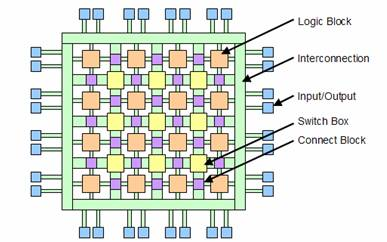
\includegraphics[width=.7\linewidth]
        {../images/fpga_architecture_abstraction_-_olin_college.jpg}
        \caption[Abstração da arquitetura de uma FPGA]
            {Abstração da arquitetura de uma FPGA.~\cite{fpga_arch_abstraction}}
        \label{fig:fpga_general_arch}
    \end{figure}

    {
        Os blocos lógicos possuem \textit{lookup tables}, registradores, somadores
        e multiplexadores. É neles que a lógica reconfigurável é implementada.
    }

    {
        Já as chaves de interconexão são responsáveis por conectar os diversos
        blocos da \textit{FPGA}. A Figura~\ref{fig:fpga_switch_box} exemplifica
        como é feito o roteamento da malha de interconexão. Os blocos de conexão
        direta são um tipo especial de chave de interconexão, e sua função é ligar
        blocos lógicos adjacentes.
    }

    {
        Por fim, as portas de entrada e saída conectam a \textit{FPGA} ao ``mundo
        externo'' e.g. \textit{drivers} de áudio e vídeo.
    }

    \begin{figure}[H]
    \centering
    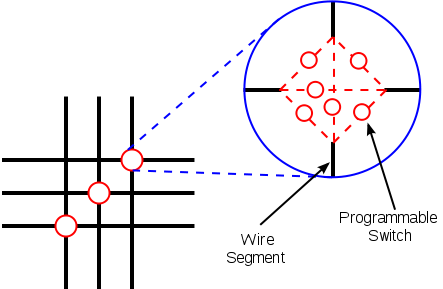
\includegraphics[width=.5\linewidth]
        {../images/switch_box_wikimedia.png}
        \caption[Funcionamento da chave de interconexão]
            {Funcionamento da chave de interconexão.~\cite{fpga_switch_box}}
        \label{fig:fpga_switch_box}
    \end{figure}


    \subsection{Arquitetura da FPGA Cyclone V SoC}
    {
        A Figura~\ref{fig:cyclone_v_arch} apresenta a arquitetura da
        \textit{FPGA Cyclone V SoC}.
    }

    \begin{figure}[H]
    \centering
    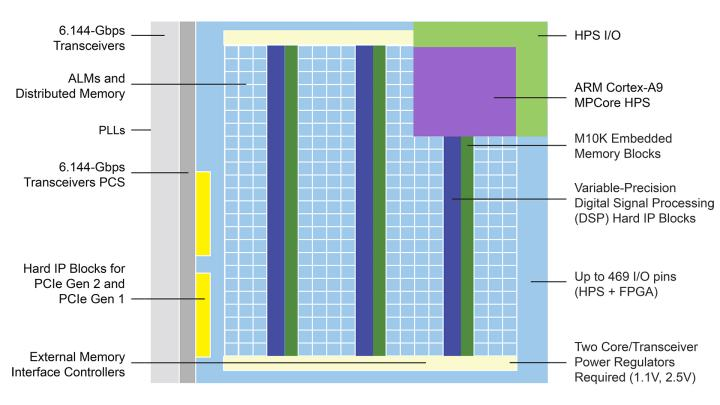
\includegraphics[width=1\linewidth]
        {../images/altera_cyclone_v_soc_architectural_downscale.jpg}
        \caption[Arquitetura da FPGA Intel Cyclone V SoC]
            {Arquitetura da \textit{FPGA Altera Cyclone V SoC} \quad Fonte: Intel}
        \label{fig:cyclone_v_arch}
    \end{figure}

        \subsubsection{Adaptative Logic Modules}
        {}

        \begin{figure}[H]
        \centering
        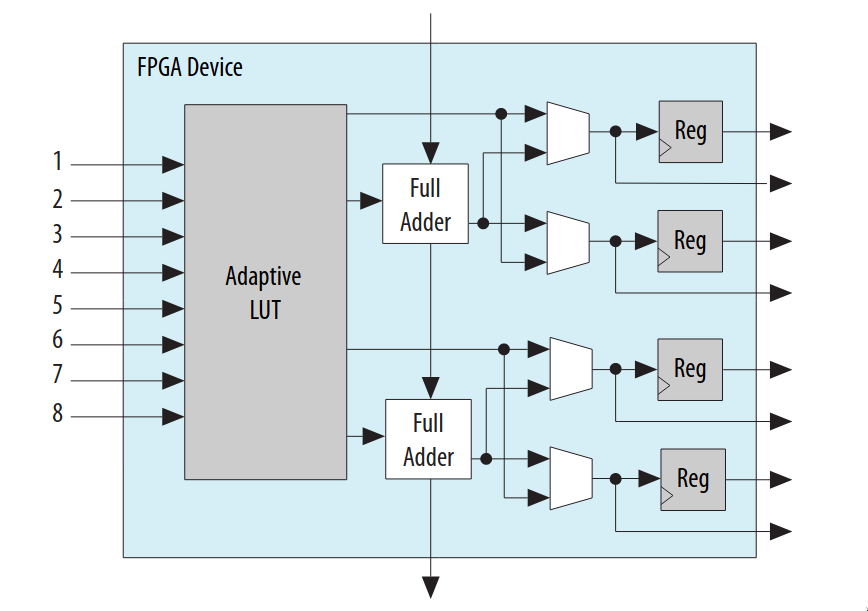
\includegraphics[width=1\linewidth]
            {../images/intel_alm_high_level.png}
            \caption[Diagrama de blocos de um ALM]
                {Diagrama de blocos de um ALM\quad Fonte: Intel}
            \label{fig:fpga_alm}
        \end{figure}


        \subsubsection{Embedded Memory Blocks}
        {}

        \subsubsection{Phase-Locked Loops}
        {}


\section{Estado da Arte dos processadores RISC-V}

